\chapter{Zero-Knowledge Proofs}
This chapter surveys selective literature about zero knowledge proofs for practical design application. The goal is to familiarize the reader with the content classification of zero-knowledge proofs in cryptography, and to give an introduction and comparison of main argument systems widely used as of today. Zero-knowledge proof systems belong to the domain of verifiable computation \citep{Simunic, Ahmad}. Verifiable computation (VC) makes use of cryptographic protocols and arguments to verify that a computation was performed correctly. Arguments allow for false proofs only if they require very high computational power. 

The introduction of interactive proof systems (IPs) by \citet{GoldwasserIPs} and \citet{BabaiIPs} shows that only correct proofs are valid and malicious proving strategies cannot be verified. Traditional proofs are static and are made for easy, step-wise computation verification, whereas IPs require interaction between prover and verifier. In computational complexity theory, interactive proof systems are abstract machines exchanging messages between prover and verifier to convince the verifier that these sets of strings belong to a language \(L\). Here, the formal language \(L\) is defining a decision problem, i.e., a computational problem that has only two outputs, yes and no. Examples of sets of strings in \(L\) can be, that a certain Bitcoin transaction is valid, \(x = 7\) for a given \(f(x)\), or a certain object belongs to a specific merkle tree. The untrusted prover has unlimited computational power and the verifier is honest and computationally restricted. Advances in computational complexity theory during that time showed that IPs are more efficient and belong to a wider class than the traditional \textbf{NP}, i.e., problems solvable in deterministic polynomial time by reading proof strings of polynomial length \citep{SassonIOPsinproceedings}. In 1987, it was shown that every language belonging to NP has zero-knowledge proof systems \citep{anymental10.1145/28395.28420}. Later, it was shown that the class of \textbf{IP}, i.e., problems solvable by interactive proof systems, lies in \textbf{PSPACE}, i.e., problems solvable in polynomial space \citep{Shamir10.1145/146585.146609}, and that every language \(L\) in polynomial time has an interactive proof system \citep{Lund10.1145/146585.146605}. The complexity class of IP describes prover and verifier interaction in a polynomial number of rounds. Other important advances in computational complexity theory are \textbf{MIP=NEXP} \citep{Laszlo} and the \textbf{PCP theorem} \citep{PCPTheorem}. These works resulted in a set of proof and argument systems, that will be introduced in this chapter. \citet{Thaler} gives a further, exhaustive overview of all systems and in-depth protocol descriptions. 

The examined proof systems are secure against computationally unrestricted provers: \textit{Interactive Proof (IP), linear Probabilistically Checkable Proof (PCP), and Interactive Oracle Proof (IOP)}. 

Combining the systems above with cryptographic tools to force certain behavior in the proof generation will create an argument system. Argument systems are considered to be zero-knowledge, if and only if the proof does not reveal anything but its own validity \citep{GoldwasserIPs}. Adding certain properties, e.g. non-interactivity, succinctness, and knowledge, will design a certain argument of knowledge, e.g. zk-SNARK (zero-knowledge succinct non-interactive argument of knowledge). Different zk-SNARKS and notions will be examined in more detail.

The next sub chapters are structured according to the design approach described above. First, IPs, PCPs, and IOPs will be defined. Through the combination with polynomial commitment schemes argument systems can be designed. Non-interactivity is achieved through Fiat-Shamir transformation. Second, properties and mathematical tools will be introduced to describe different arguments of knowledge: zk-SNARK, FRI-STARK and bulletproofs. Third, real-world applications of zero-knowledge proof systems will be summarized. Lastly, the different proof systems will be evaluated in different application scenarios.

\section{From Proof Systems towards Argument Systems}

A mathematical proof in the context of computer science and cryptography is any object that convinces a verifier that a statement is correct. Mathematical proofs embody what is defined in the complexity class NP. A proof system is a structured scheme that outputs a decision of whether a statement is correct or incorrect. In general, there are three properties that are desirable for proof systems \citep{GoldwasserIPs}, which will be introduced shortly. Throughout this chapter, these properties will be revisited more exhaustively.
\begin{itemize}
    \text{\parbox{420pt}{
    \item The procedure to create and verify proofs should be \textbf{efficient and fast}. 
    \item \textbf{Completeness}: True statements should have a convincing proof of their validity.
    \item \textbf{Soundness}: If a statement is incorrect, there is no possibility of it having a convincing proof.}}
\end{itemize}
Unlike argument systems, proof systems do not limit the malicious prover in its computational power (\textit{statistical soundness}). Using cryptographic primitives and restricting the prover, e.g., probabilistic polynomial time proof, so that it cannot break the primitives, describes the design towards argument systems, which are computationally sound \citep{ArgSystems, MicaliArgSys}. Each proof system presented makes assumptions on the prover. However, only with the use of cryptographic tools and zero-knowledge, these proof systems can be extended with additional properties to yield zero-knowledge argument systems of various kinds.

\begin{comment}
IPs are the basis to understand cryptographic protocols and argument systems
argument systems are IP with a specific assumption
polynomial IOPs together with polynomial commitment scheme always yields a specific argument of knowledge, can be made non interactive with fiat-shamir, can be succinct too, different abwandlungen
but before we need basic understanding on different proof systems that lie behind the construction of argument systems
then we need understanding of commitment scheme and fiat shamir transform
how zero knowledge is applied in the design will be shown later when going through the different systems

information secure = only theoretically
what are those, little history
1:polynomial IOPs 
- interactive proofs intro
- MIPs
- constant round IOPs
2:linear PCPs
-intro from the book Thaler-->combined with cryptographic primitives we get SNARKs, everything is a SNARK and SNARK variation
-Luong and Park: properties intro
- Yang Yang et al properties
-Soonhyeong 2021: better verification with EVM to verify non-maliciousness of blocks (zKSNARKS used)
\end{comment}

\subsection{Interactive Proofs}

In interactive proof systems, the prover with unlimited computational resources interacts with a computationally bound verifier in order to convince the verifier of the correctness of a statement. The verifier randomly challenges the prover, which is referred to as coin tosses \citep{GoldwasserCoinTosses}. These challenges happen in rounds, until there are sufficient tests run and the verifier is convinced. \citet{GoldwasserIPs} defined an interactive proof system that is private, i.e., that the verifiers challenges are not publicly accessible, whereas the interactive proof system of \citet{BabaiIPs} allows the coin tosses to be publicly accessible by the prover.
\begin{align*}
    \text{\parbox{450pt}{\textbf{Interactive Proof System.} \textit{\(L\) is a language over \(\{0,1\}^n\), with n representing the input size domain of n-bit strings. An interactive protocol is a interactive proof system if after \(k\) rounds, the probabilistic verifier in polynomial time exchanged \(k\) messages with the computationally unrestricted prover, and has to either accept or decline the correctness of the prover's proposition. IP is the complexity class of problems solvable by a k-round interactive proof system.}}}
\end{align*}
The transcript is the order in which messages are exchanged. The prover and verifier are functions \(P(x), V(x)\) with common input \(x\). The overall distribution of all transcriptions between prover and verifier is called \(View_V(P(x), V(x))\), which is bound by the number of rounds between \(P\)and \(V\). \(P\) provides a result that satisfies the proposition, e.g., \(y\) to a function \(f(x) = y\). \(P\) and \(V\) exchange a transcript of messages \((m_1, m_2, m_3, ..., m_k)\), whereby both parties take turns and the last message is sent by the prover. Note, that \(V\) is probabilistic with internal randomness \(r\). Hence, the output depends on \((V, x, r, P)\) and is \(\{0,1\}\), i.e., \(1\) if the statement is correct, and \(0\) if it is incorrect \citep{GoldwasserIPs, BabaiIPs}. Interactive proof systems have completeness error \(\delta_c\) and soundness error \(\delta_s\) . For any input \(x\), there must be a convincing proof that \(f(x)\) is correct. Incorrect statements for \(y \neq f(x)\) cannot result in a convincing proof, i.e., a malicious prover does not exist IP systems are valid if \(\delta_c, \delta_s \leq 1/3\) \citep{Thaler}. IPs with \(k\) provers are multi-prover interactive proofs (MIPs), introduced by \citet{MIPsBen}, and extended by \citet{MIPsSetty} to allow for the design of succinct arguments. MIPs are characterized by no information sharing and non-adaptivity of provers. The probabilistic polynomial time verifier acts similarly as in IPs, but the challenges sent are not shared among the different provers. The prover's response \(i\) does not depend on the \(i-1\) interactions in the transcript, i.e., the prover cannot react based on the previous messages, because there is at least another prover \(p_j\) whose messages are not known to \(p_i\) for \(i\neq j\) .

\begin{comment}
Some definitions are still missing:
randomness
completeness
soundness
statistical soundness
computational soundness
\end{comment}

\subsubsection{Non-interactive, publicly verifiable arguments}
The \textit{Fiat-Shamir transformation} takes any interactive proof system based on public coin tosses and transforms it into a non-interactive, publicly verifiable system. This transformation can be described effectively with the use of an ideal cryptographic assumption called \textit{Random Oracle Model (ROM)}. 
\subsubsection{Random Oracle Model}
The ROM methodology was introduced in cryptographic theory to satisfy the goal of designing secure cryptographic protocols. First, an ideal system is designed, whereby all parties have access to an oracle, i.e., a public random function. Once the security of the protocol is proven, the random oracle function is replaced by a cryptographic hashing function to implement the system in practice \citep{ROMBellare}. In IPs, the random oracle function is part of the view, i.e., random choices of challenges simulator output. It is assumed that prover and verifier can query the random oracle function \(f_R\) by sending an input \(x\), so that the random oracle returns \(f_R(x)\). In ROM, the efficiency is dependent on x, i.e., for every input in the problem size domain \(D\) , \(f_R(x)\) is captured. Since it is only practical in theory, because \(|D|\) is large to ensure security, e.g., \(2^{256}\), hash functions are used in practice \citep{ROMBellare, Thaler}, e.g., POSEIDON or SHA-3. The ROM is controversially discussed in retrospective: On the one hand, it is argued that there exist protocols that are only secure in the random oracle model and all implementation efforts in practice have led to insecure protocols, whereby the security of the ideal scheme is not maintained. The area of work at focus are digital signatures and public-key encryption, showing that the ROM is not sound \citep{ROMCanetti}. On the other hand, this conclusion is discussed to indicate there is no evidence of practical security weaknesses if there is a need for random oracle systems in a protocol. This statement is supported by protocol design examples, e.g., Elliptic Curve Digital Signature Algorithm, ECDSA, that have led to cryptographic insecurity without the use of a random oracle \citep{ROMretroKoblitz}. 
\subsubsection{Fiat-Shamir Transformation}
The Fiat-Shamir transformation \citep{ROMFiat1986HowTP} removes the need for prover-verifier interaction in a public coin interactive proof system with the help of the random oracle function. The result is a non-interactive, publicly verifiable system. IPs send messages between prover and verifier, whereby the verifier challenges the prover at random. Every message sent by the verifier in the IP is replaced by values obtained by querying the random oracle. The query always depends on the previous message sent by the prover to prevent soundness attacks. In summary, the prover only sends one message containing the transcript, i.e., the list of all messages sent by the prover and the query results of the random oracle. The input x has to be appended to the list every round. The verifier's coin tosses are not needed any longer, and there is no need for the verifier to send messages to the prover (see Figure \ref{fig:FST}).

\begin{figure}[hbt]
	\centering
		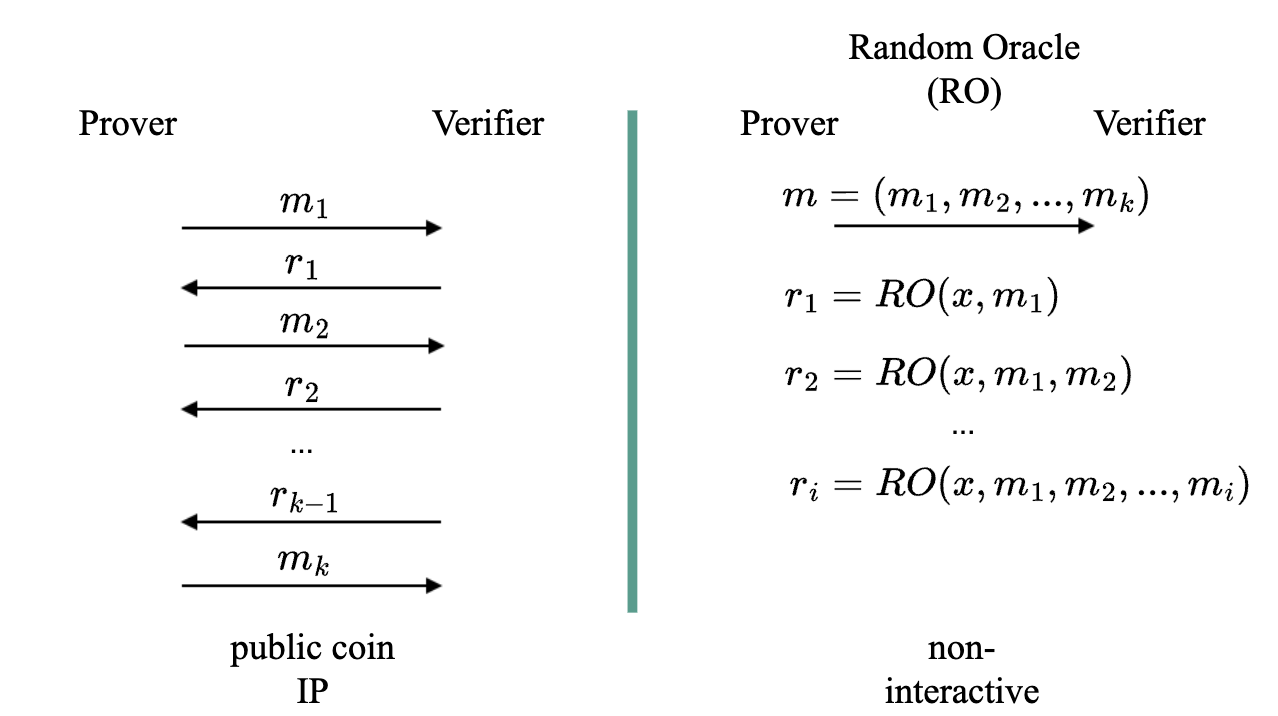
\includegraphics[width=0.8\textwidth]{Pictures/FST.png}
	\caption{Generic Fiat Shamir Transformation illustrated (based on \citet{Thaler})}
	\label{fig:FST}
\end{figure}
Argument systems are obtained by applying polynomial commitment schemes to proof systems, whereby the prover commits to a low-degree polynomial. It allows for polynomial evaluation verification without possessing all the information of this polynomial.  Polynomial commitment schemes are used to proof that a polynomial, evaluated at a specific input results in a specific output. The prover commits to the polynomial, which can be perceived as some object hiding the polynomial, e.g., similar to a hash. The verifier challenges the commitment with a random value. The committer then creates a proof that the polynomial evaluates at that random value at a specific point. The polynomial itself is not revealed. In interactive proof systems with an honest prover running in polynomial time, e.g., GKR protocol, any arithmetic circuit can be evaluated \citep{GKR10.1145/1374376.1374396}. Arithmetic circuits have gates that operate on two types, i.e., addition and multiplication. Besides gates, there are wires, that carry integer variables. Retrospectively, it is an important achievement, since arbitrary computer programs can be expressed via arithmetic circuits, which is the basis layer of many zero-knowledge protocols as of today. More mathematical tools for understanding the functionality of argument systems are covered in chapter 5.2.
\subsubsection{Zero-Knowledge}
If the verifier knows nothing about the statement and the witness, but its validity, the algorithm will run in zero-knowledge. This property can be described by making use of a simulator notion \citep{Thaler}: There exists a prover and probabilistic polynomial time verifier strategy under the honest verifier assumption. For any probabilistic polynomial time verifier strategy, there is a probabilistic polynomial time algorithm (simulator), that can depend on the verifier strategy, which produces outputs that are indistinguishable from the distribution of transcripts generated through the prover and verifier strategy interactions. The simulator ensures, that the verifier only learns that \(x \in L\). Under the honest verifier assumption, there are at least six types of zero-knowledge protocols, whereby the notion of simulator output and transcript distribution being indistinguishable is at focus \citep{zktypes}:
\begin{itemize}
    \item \textbf{Perfect Zero-Knowledge}: The output of the simulator \(S(x)\) and the distribution of the transcript created through prover and verifier strategy interaction \(View_V(P(x), V(x))\) within the protocol is identical. 
    \item \textbf{Statistical Zero-Knowledge}: \(S(x) \text{ and } View_V(P(x), V(x))\) have a negligible statistical distance, given a polynomial number of samples from the distributions.
    \item \textbf{Computational Zero-Knowledge}: \(S(x) \text{ and } View_V(P(x), V(x))\) can be distinguished with negligible probability, only if a polynomial number of samples is given.
\end{itemize}
Resuming the definition in 5.1, soundness is divided into statistical (for proof systems) and computational (for argument systems) soundness. Argument systems are computationally sound, i.e., allow for applying cryptographic primitives. The computationally bound prover cannot break these primitives, unlike the unbound prover in proof systems, which are statistically sound \citep{Thaler}. The verifier not only learn that a statement is true, but also has to be convinced that the prover knows a witness that is true. The simulator is able to extract that witness information through interaction with the algorithm (knowledge soundness) \citep{NitulescuGentleIntroSNARKs}.

\subsection{Linear PCPs}
\textit{Probabilistically Checkable Proofs} (PCPs) differ from previously introduced proofs, because there is no need for the prover to answer queries based on the current or previous query content posted by the verifier. The polynomial time verifier is provided with oracle access to a static proof string \begin{math} \pi \end{math}, whereby the proof is queried and the result of it only depends on the currently processed query \citep{PCP}. The breakthrough of powerful, pairing-based schemes is attributable to \citet{GennaroLinPCP}, who introduced \textit{Quadratic Arithmetic Programs} (QAPs), as variant of quadratic span programs. Quadratic span programs are more efficient, because they only satisfy boolean circuits. Therefore, the introduction of QAPs is important to represent more practical computations, e.g., multiplication gates, whereby the efficiency lies in the usability for effectively solving more natural problems. Any arithmetic circuit instance can be transformed into instances of a \textit{rank-1 constraint system} (R1CS).
\begin{align*}
    \text{\parbox{450pt}{\textbf{R1CS.} \textit{A R1CS is an intermediate representation of the computational problem, which is used to perform the application of argument systems. Given a set of \(n \times m \text{ matrices} \ A, B, C\), with values derived from a finite field \begin{math} \mathbb{F} \end{math}. A R1CS instance is called satisfiable, if there exists a solution vector \(z \in\) \begin{math} \mathbb{F}^n \end{math} with \(z_1 = 1\), so that}}}
\end{align*}
\begin{align*}
    (A \cdot z) \circ (B \cdot z) = C \cdot z.
\end{align*}
For every \(i\)th row each of the three matrices, belonging to the finite field circuit size, the following equation must hold true:
\begin{align}
    \langle a_i, z \rangle \cdot \langle b_i, z \rangle - \langle c_i, z\rangle = 0 
\end{align}

In practice, \(z\) is known by the prover. The solution vector also has a public input, namely the result to a computation (refer to chapter 6.1 for example calculations). The goal is to arrive at an univariate polynomial \(t(x)\), when divided by the minimal polynomial, represents a secret polynomial \(h(x)\) without remainder. The minimal polynomial is always known, if the number of constraints are known, and is a multiple of \(t(x)\). In the linear PCP, (5.1) is evaluated in linear, constant time. The QAP is obtained by taking each value of each row of the R1CS matrices as output of a polynomial, which is to be calculated. The polynomial results to that specific value in the R1CS, when evaluated at \(X = \{1, 2, ..., \text{number of constraints}\}\). Given these constraints, the three sets of polynomials are calculated via the sum of \textit{Lagrange Interpolation}.
\begin{align*}
    \text{\parbox{450pt}{\textbf{Lagrange Interpolation.} \textit{The polynomial obtained through Lagrange Interpolation is the polynomial \(P(x)\) of degree at most \(\leq (n-1)\) and passes through the n points \((x_1, y_1 = f(x_1)), (x_2, y_2 = f(x_2), ..., (x_n, y_n = f(x_n))\), that are given. It is denoted by}}}
\end{align*}
\begin{align}
        P(x) = \sum_{j=1}^{n} P_j(x)
\end{align}
\begin{align*}
        P_j(x) = y_j * \prod_{\substack{k = 1 \\ k \neq j}}^{n}\frac{x-x_k}{x_j-x_k}
\end{align*}
\begin{align*}
    \text{\parbox{450pt}{\textbf{Example.} \textit{Let \(n = 2\) with the three given points \([1,0], [2,1], [3,0]\). The polynomial obtained through Lagrange Interpolation is: 
    }}}
\end{align*}
\begin{align*}
    P(x) = \sum_{j=1}^{2}\left(y_j*\prod_{\substack{k = 1 \\ k \neq j}}^{n}\frac{x-x_k}{x_j-x_k}\right)
    &= 0 * \frac{(x-2)(x-3)}{(1-2)(1-3)}+1*\frac{(x-1)(x-3)}{(2-1)(2-3)}\\
    &= 0 * \frac{(x-1)(x-2)}{(3-1)(3-2)} = \frac{x^2-4x+3}{-1}\\
    &= -x^2+4x-3
\end{align*}
Each gate is the \(x\) value and the values of the R1CS matrix column are the corresponding \(y\) values for the computation, so that the QAP can be obtained. It consists of three sets of polynomials (see chapter 6.1 for example calculations). Each interpolation calculation receives n points (number of constraints), and the result is a polynomial of degree \(n-1\). Multiplying each polynomial in the matrices with the solution vector yields the final polynomials \(A(x), B(x), C(x)\), whereby 
\begin{align}
    \frac{A(x) * B(x) - C_(x)}{Z(x)} = H(x).
\end{align}
In a linear PCP, the proof consists of evaluations of linear functions, which is created by the prover. Soundness is guaranteed against a dishonest prover by ensuring that the proofs are relying on a specific structure. The verifier is querying the proof. By transforming linear PCPs into non-interactive argument systems, the trusted setup issues proving and verifying keys, which are used to perform checks using pairing-based cryptography. Many systems rely on this feature, e.g., Groth16, whose mathematical tools and general protocol procedures are presented in 5.2.1.

\subsection{constant round IOPs}
\subsection{Polynomial IOPs}
%(focus on chapter 10.6, combine with preliminaries from previous chapters in Thaler)

The proof systems introduced in this chapter form the base layer of zero-knowledge succinct, non-interactive arguments of knowledge. The proof is convincing and the witness is valid, while the verifier learns nothing about it except for its validity and cannot be convinced by an invalid witness (completeness, soundness and zero-knowledge). The zero-knowledge IPs by \citet{GoldwasserIPs} described in 5.1.1 were the begin of research and implementations towards zk-SNARKs.

\section{Zero-knowledge succinct, non-interactive arguments of knowledge}
Following the first zero-knowledge IPs \citep{GoldwasserIPs}, \citet{Blum1991} introduce the common reference string (CRS) and create non-interactive zero-knowledge proofs with only one message to be shared, i.e., the proof. Subsequently, research on reducing the proof size increased, \citet{MicaliArgSys} introduces the first non-interactive zero-knowledge proof with sublinear proof size. Building on these findings, the first zk-SNARKs for circuit satisfiability uses proofs that are constant-size and uses pairings to efficiently check the polynomial equations without revealing any information, e.g., coefficients \citep{Groth2010ShortPN}. \citet{GennaroLinPCP} continue with increasing the efficiency of polynomial equation verification and introduce QAPs. \citet{Pinocchio} makes use of it and develops the Pinocchio protocol, that utilizes QAPs and the knowledge of coefficients to efficiently verify polynomial equations through eight pairing checks without revealing any decodings. This protocol is enhanced by \citet{Groth2016OnTS}, reducing the proof size again and decreasing the number of pairing checks to three. It is widely used as of today and the characteristics of succinctness and non-interactivity make it particularly useful in blockchain, e.g., in Zcash and Circom \citep{chen2022review}. In the following, different zk-SNARK designs will be defined. Current research focuses on quantum resistant systems \citep{chen2022review}, hence, FRI-STARK and bulletproofs will be introduced as well. 

\begin{comment}
- Chen et al (2022) very good paper for this
- what is zero knowledge definition
- what means indistinguishable
- different types of zero-knowledge (perfect, statistical, computational)
-first succinct argument of knowledge by goldwasser etc. 
-what is succinct
- repeat that Fiat Shamir Transformation can make them all non-interactive
-every proof from above combined with polynomial commitment schemes yields a SNARK
-short explanation what are polynomial commitment schemes: %https://coingeek.com/how-plonk-works-part-1/#:~:text=PLONK%20is%20a%20state%2Dof,by%20all%20circuits%5B1%5D.
- how: 1 design a public-coin polynomial IOP for circuit- or R1CS-satisfiability, 2 use polynomial commitment scheme 3 remove interaction via fiat shamir
- linear PCPs are exception: they need to be combined with pairing based cryptography
- everything is a sub of SNARKs
- I only want to cover three most practical zero knowledge SNARKs
- Constant-round IOPs vs. MIPs and IPs-->p.301 Thaler
- every combo with polynomial commitment scheme is a SNARK
- we focus on Groth16, PLONK, FRI-STARK, bulletproof
\end{comment}

\subsection{Circuit-specific zk-SNARK from QAP}
With the introduction of QAP by \citet{GennaroLinPCP} as starting point, \citet{Groth2016OnTS} introduced an important and most performative zk-SNARKs for circuit satisfiability. The linear interactive proof (LIP) provided reduces the number of verifier queries to three, and the number of group elements from ten to six. Previous security relied on the Knowledge of Exponent Assumption (KEA), which was enhanced by establishing security in the generic group model. Practically, the Fast Fourier Transform (FFT) is utilized. Changing the circuit to a small degree still requires a complete restart of the trusted setup \citep{Thaler}. In the following, preliminary assumptions and definitions for designing circuit-specific zk-SNARKs from QAP are introduced, providing a starting point of the functionalities in the Groth16 protocol applied in 6.2.
\begin{align*}
    \text{\parbox{450pt}{\textbf{Linear Interactive Proof (LIP).} \textit{While linear PCPs ensure that the prover answers any verifier query through a linear function, LIPs ensure soundness against provers that do not use the same linear function to answer queries. Any linear PCP can be transformed to LIP \citep{bitansky}. The Knowledge of Exponent Assumption (KEA) guarantees, under the hard discrete logarithm problem, that the prover in fact is knowledgeable about these linear functions, i.e., can proof that the same coefficients are used for all polynomials resulting from the QAP.}}}
\end{align*}
SNARKs from QAP consist of a generation algorithm, prover, and verifier \citep{Groth2016OnTS, Guo}BENAMARA, which are introduced informally.
The generation algorithm executes the trusted setup by taking a random security parameter and the arithmetic circuit as input. The QAP is generated over a finite field, which forms the basis for the trusted setup run. With secret states and parameters not to be known by anyone and deleted after (toxic waste), the CRS is created as an output of the generation algorithm (for detailed structure, see 6.2). The prover algorithm uses the CRS and public statements to compute a witness, so that the target polynomial, i.e., result of encoded computation from QAP, and the minimal polynomial vanish on some quotient polynomial. After it has been ensured, the proof is generated. The proof consists of elements resulted from the encoded computation, generated by two group elements. The verifier algorithm uses the proof and performs pairing checks to output either a true or false. In Groth16, the pairing checks are minimal and the parameters and generated values are mainly taken from the proving and verification key (6.2). Perfect completeness is achieved if a true statement is known by the prover, because an honest verifier will be convinced \citep{Guo}. Zero-knowledge is achieved by randomizing the polynomials and uniformly distribute the proof terms \citep{Groth2016OnTS, Groth2010ShortPN}.

The combination of linear interactive proofs with pairing-based cryptography is particularly useful due to the functionality of bilinear maps (6.2). Through the use of bilinear maps, one homomorphic multiplication operation can be executed:
\begin{align*}
    \text{\parbox{450pt}{\textbf{Bilinear Maps and Multiplicative Homomorphism.} \textit{Given the commitments \(a_1, a_2, a_3\) and the values \(b_1, b_2, b_3\) in the commitments, and the bilinearity of the following map \begin{math}
        e: \mathbb{G} \times \mathbb{G} \to \mathbb{G}_t
    \end{math}, \(e(g^{b_1}, g^{b_2}) = e(g^{b_3}, g)\), if and only if \(b_3 = b_1 * b_2\).}}}
\end{align*}
In practice, \begin{math} \mathbb{G} \end{math} is an elliptic curve group defined over prime finite field \begin{math} \mathbb{F}_p \end{math}, and \begin{math} \mathbb{G}_t \end{math} is a subgroup of the extension field of \begin{math} \mathbb{F}_p \end{math}, namely \begin{math} \mathbb{F}_{p^k} \end{math}. \(k\) is a positive integer and defines the embedding degree of the elliptic curve group, and must be low to efficiently apply pairings. If \(k\) is too large, the mapped elements to \begin{math} \mathbb{G}_t \end{math} will be more expensive to operate on \citep{Thaler}.
\begin{align*}
    \text{\parbox{450pt}{\textbf{Decisional Diffie-Helman Assumption (DDH).} \textit{Given a cyclic group \begin{math}\mathbb{G}\end{math} with generator \(g\) and \(g^a, g^b\) for \(a, b\)}, chosen uniformly and independently from \begin{math}\mathbb{G}\end{math}, \(g^{ab}\) is computationally indistinguishable from a random group element of the cyclic group.}}
\end{align*}
Instead of KEA, the FFT can be used to compute the Decisional Diffie-Helman problem more efficiently, in \(O(nlogn)\). This is achieved by making use of roots of unity. The element \(w\) is a root of unity in finite field \begin{math} \mathbb{F}\end{math}, whereby \(w^n = 1\) with \(n\) being the \(n^{th}\) primitive root of unity for all positive integers s smaller than \(n\), \(w^s \neq 1 \). Instead of evaluating a polynomial at \(n\) point pairs \(\{(x_0,y_0), (x_1,y_1), ..., (x_{n-1}, y_{n-1})\}\), the values \(1, w, w^2, ..., w^{n-1}\) are used, halving the values to \(\frac{n}{2}\) \citep{Groth2016OnTS}.

\subsection{Permutation argument zk-SNARK}
\textit{Permutations over Lagrange-bases for Oecumenical Non-interactive Arguments of Knowledge} (PLONK) is a zk-SNARK with a universal trusted set-up, which produces a \textit{structured reference string} (SRS). The SRS is of size \(d\), used for circuits of up to \(\leq d\) gates. This universal SNARK has fully succinct verification and low prover run time \citep{PLONKcryptoeprint:2019/953}, compared to its predecessor Sonic \citep{SONIC10.1145/3319535.3339817}, which was the first universal and fully succinct SNARK. PLONK is based on constant round polynomial IOP and uses the polynomial commitment scheme based on \citet{Kate2010ConstantSizeCT}. It is presented as a non-interactive protocol, obtained through Fiat-Shamir transformation \citep{PLONKcryptoeprint:2019/953}. The trusted setup is universal and updatable: it can be used for the entire scheme and does not have to be produced for every problem (circuit), e.g., in Groth16. Also, the Kate commitment scheme can be replaced by any other polynomial commitment scheme, e.g., FRI (see chapter 5.2.3). 
Kate commitments use the elliptic curve generated points published in the public key after trusted setup, similar to Groth16 (see chapter 6.1 for detailed description), to commit to a polynomial of degree \(d\). The first \(d+1\) points are used to evaluate the polynomial at the respective coefficient. The underlying assumptions can be attributed to the \textit{Schwartz-Zippel lemma}.
\begin{align*}
    \text{\parbox{450pt}{\textbf{Schwartz-Zippel Lemma.} \textit{Let \(f(x)\) be a non-zero polynomial with degree \(d\) over \begin{math}\mathbb{F}^n\end{math}, then, for a randomly chosen \(r\), the probability of \(f(r) = 0\) is at most \(\frac{d}{n}\).}}}
\end{align*}
The \textit{Schwartz-Zippel lemma} proves that the polynomial evaluates to 0 at any point with high probability, if it evaluates to 0 at a given random \(r\). If two polynomials evaluate equally at \(r\), they are equal at every point with high probability. In a polynomial commitment scheme this suggestion is beneficial. The prover evaluates the polynomial at the random \(r\) chosen by the verifier, and sends it along with a proof. If the proof is valid, the verifier concludes that the result of the prover is also valid \citep{Kate2010ConstantSizeCT}.

The computation is first converted into an arithmetic circuit. Then, the arithmetic circuit is used to obtain a constraint system, similar to the R1CS from the previous chapter. Both have only one multiplication allowed per gate. However, PLONK only allows for one addition per gate, as long as it is not a constant. This constraint system also comes with copy constraints, which are used to transform the system into polynomials. The verification is executed using a polynomial commitment scheme (see Figure \ref{fig:plonk}).

\begin{figure}[hbt]
	\centering
		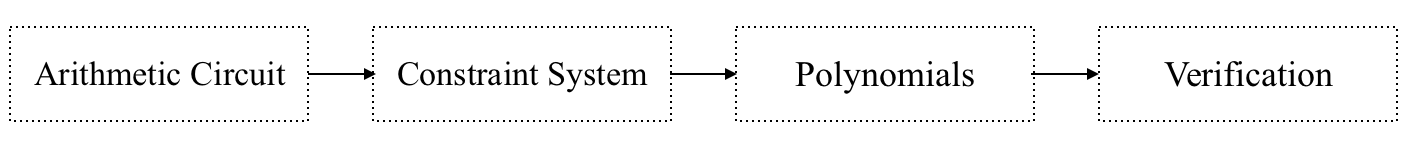
\includegraphics[width=0.8\textwidth]{Pictures/plonk_process.png}
	\caption{PLONK steps (simplified)}
	\label{fig:plonk}
\end{figure}

Similar to circuit-specific zk-SNARKs, e.g., Groth16, the computation has to be flattened for the protocol to process it. The problem is represented in an arithmetic circuit, consisting of gates that can be either representing an addition or a multiplication. Then, the arithmetic circuit is transformed into a constraint system representing the wires of the circuit. In analogy to circuit-specific zk-SNARKs, the constraint system is dependent on the number of gates (see chapter 6.1 for a simple example implementation). In PLONK, the constraint system is normalized into a specific form, which will be presented shortly, and is referred to as part of the public input in \citet{PLONKcryptoeprint:2019/953}. 
It is distinguished between constraints per gate and constraints across gates in the arithmetic circuit. The formalization system of gate constraints is the following:

\begin{align}
    Q_{L}a + Q_{R}b + Q_{O}c + Q_{M}ab + Q_C = 0
\end{align}

\(L, R, O\) represent the left, right and output gate wire. \(M, C\) stand for multiplication and constant. This standardized form allows representation of addition and multiplication. Setting \(Q_{M}ab = 0, \ Q_C=0, \ Q_{O}c = -1 \) and the rest to 1 will represent \(a + b - c = 0\). Setting \(Q_{L}a =1,\ Q_{L}b =1,\ Q_{O}c = -1\) and the rest to 0 will represent multiplication. Each gate is represented in the form presented in 5.1. Similar to the R1CS previously described, \(Q_{L}a, Q_{L}b, Q_{O}c, Q_{M}ab, Q_C\) can be expressed as vectors that hold the circuit structure. Again, in analogy with the R1CS, \(a, b, c\) can be expressed as vectors as well, which are the witness assignments. In correlation to chapter 5.2.1, these witness assignments might be private and only known to the prover.
In this constraint system, there are vectors \(Q_{L}, Q_{L}, Q_{O}, Q_{M}, Q_C, a, b, c\). Using the indices of these vectors as x, they can be transformed into polynomials of evaluation format. As an example, let us define one of the vectors in a circuit with 4 gates to illustrate the procedure. 

\begin{align}
    Q_L = (1,0,1,0) \text{ converts into the set of points } {(0,1), (1,0), (2,1), (3,0)}.
\end{align}

The set of points matches a degree 3 polynomial, which can be shown in a coordinate system (see Figure \ref{fig:examplepoly}). Through Lagrange Interpolation, the concrete polynomial in coefficient form can be calculated. 
\begin{figure}[hbt]
	\centering
	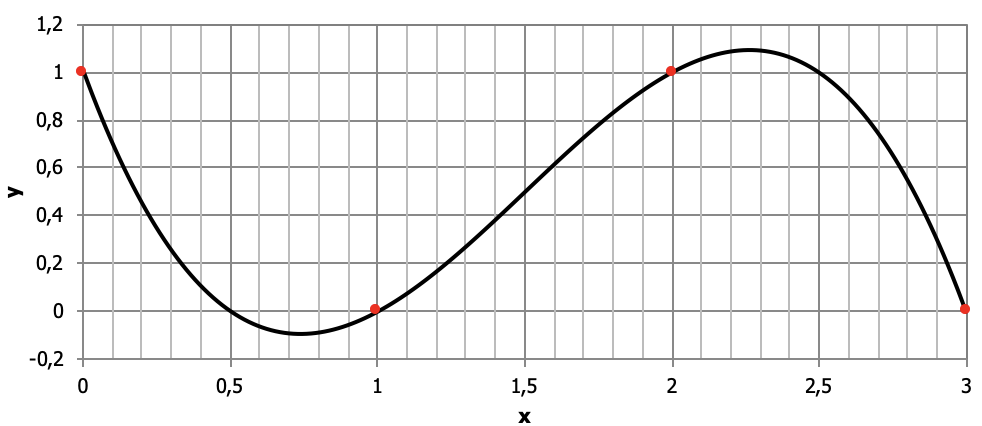
\includegraphics[width=0.6\textwidth]{Pictures/example_polynomial.png}
	\caption{Example polynomial \(Q_{L}(x)\) evaluated at the points in 5.2. Lagrange Interpolation yields coefficient form \(Q_{L}(x) = - 0.6667x^3 + 3x^2 - 3.3333x + 1\)}
	\label{fig:examplepoly}
\end{figure}

This procedure is applied to all Q-vectors and the vectors a, b, c to transform them from constants into polynomials. The corresponding function obtained is
\begin{align}
    f(x) = Q_{L}(x)a(x) + Q_{R}(x)b(x) + Q_{O}(x)c(x) + Q_{M}(x)a(x)b(x) + Q_{C}(x) = 0\\
    f(x) = Z(x)H(x)
\end{align}

This will allow to compress as much information as possible into a single source, i.e., a polynomial. 

Besides the constraints as per gate, there are also constraints that hold across gates, e.g., the output of a gate can be equal to the input on another gate. It is necessary to represent them too, in order to translate the whole problem into the scheme. These copy constraints can lie within one vector, e.g., if \(b0 = b2\), or between multiple vectors, e.g., \(c0 = a3 = b1\). In the first case, the indices of the vectors are exchanged to create a permutation function \(\sigma(i)\). In the second case, the vectors are combined into one long vector, before the permutation function is obtained. Once all copy constraints are generated as lists of permuted indices, they are transformed into polynomials of the permuted gate indices. The resulting polynomials are
\begin{align}
    \sigma_{a}(x), \sigma_{b}(x), \sigma_{c}(x)
\end{align}

A proof is generated by using these permutations and computing the values of all the gates to create the polynomials of \(a(x), b(x), c(x)\). Now, an accumulator \(p(x)\) will be designed in order to represent all coordinates in the set of points between the vectors \(a, b, c\). It proves the copy constraints as follows.
\begin{align}
    p(x+1) = p(x) * (v_1 + X(x) + v_2 * Y(X))
\end{align}
\(v_1, v_2\) are random values and \(X, Y\) are polynomials per vector representing the x and y coordinates. For every copy constraint, e.g., \(a1=a3\) or \(b4=c1\), there will be a \(X(x)\) representing the x coordinates \(a,b ,c\) (note, these are the indices introduced (5.2). \(X'(x)\) will be a polynomial representing the indices flips in the copy constraint. Every vector will be represented in \(p_{a}(n), p_{b}(n), p_{c}(n)\) and \(p'_{a}(n), p'_{b}(n), p'_{c}(n)\). Instead of checking each copy constraint within the same vector individually, the following multiplication check is performed to also check copy constraints across vectors at the same time:
\begin{align}
    p_{a}(n) * p_{b}(n) * p_{c}(n) = p'_{a}(n) * p'_{b}(n) * p'_{c}(n)
\end{align}
In practice, the permutation accumulators are not expressed in dependency of vector size \(n\), but through high order roots of unity, whereby the field elements satisfy \(\omega^n = 1\). Also, all values are expressed as elements within a finite field of prime order \(p\), similar to the circuit specific zk-SNARKs. The X coordinates are not expressed as indices dependent of vector size \(n\), but with \(omega\) and some random element \(g\) in the field.
\subsubsection{Summary}
After transforming all the constraints intro sets of polynomials, the following checks need to be performed to verify the proofs \citep{PLONKcryptoeprint:2019/953, buterinplonk, chen2022review}. Through the polynomial commitment scheme based on \citep{Kate2010ConstantSizeCT}, these checks can be verified. Elliptic curve points are generated at random, similar to circuit based zk-SNARKS, and used to evaluate the polynomials. Elliptic curve pairings allow to check whether the equations hold true without any of the generated points, or polynomials to be revealed. 
The equation in (5.3) is the main equation of the circuit that needs to be checked. Then, in total, there are six permutation accumulator functions for the witness assignment vectors and their copy constraints. The equation check in (5.4) is resulting into six rounds:
\begin{align}
    P_{a}(\omega x) - P_{a}(x)(v_1 + x + v_2a(x)) = Z(x)H_{1}(x) \\
    P_{a'}(\omega x) - P_{a'}(x)(v_1 + \sigma_{a}(x) + v_2a(x)) = Z(x)H_{2}(x) \\
    P_{b}(\omega x) - P_{b}(x)(v_1 + gx + v_2b(x)) = Z(x)H_{3}(x) \\
    P_{b'}(\omega x) - P_{b'}(x)(v_1 + \sigma_{b}(x) + v_2b(x)) = Z(x)H_{4}(x) \\
    P_{c}(\omega x) - P_{c}(x)(v_1 + g^{2}x + v_2c(x)) = Z(x)H_{5}(x) \\
    P_{c'}(\omega x) - P_{c'}(x)(v_1 + \sigma_{c}(x) + v_2c(x)) = Z(x)H_{6}(x)
\end{align}

There are constraints for the accumulator to be checked which result from (5.7):
\begin{align}
    P_{a}(1) = P_{b}(1) = P_{c}(1) = P_{a'}(1) = P_{b'}(1) = P_{c'}(1) = 1 \\
    P_{a}(\omega^n)P_{b}(\omega^n)P_{c}(\omega^n) = P_{a'}(\omega^n)P_{b'}(\omega^n)P_{c'}(\omega^n)
\end{align}

The only program specific polynomials that need to be computed upfront by prover and verifier are the \(Q\)-polynomials from the circuit and the \(\sigma\)-permutation polynomials. The verifier algorithm only stores commitments to these polynomials. The user inputs are the witness assignments \(a(x), b(x), c(x)\), the accumulators \(P\) from above and the different \(H\) for every round. Although the verification is efficient, the proof size is still an area of improvement. For the implementation of plonk in circom and snarkjs, see chapter 6.2.2.

\subsection{FRI-STARK}
\begin{comment}
with FRI-based polynomial commitment
-does not use R1CS
-fri starks
-Salleras et al 2021
\end{comment}

\subsection{Bulletproofs}
\begin{comment}
with discrete-log based polynomial commitment
- uses R1CS too
- they are non-interactive,
- they are zk arguments of knowledge
- Godden et al bulletproofs
- Chung et. al bulletproof+
- Deng at al history of bulletproofs
-Salleras et al 2021
main protocols: Lipmaa, Boudot, then Groth and Coutueau, then Hybrid from Kim Lee 2019
Deng et al 2022: history of range proofs, cuproof as example
-Kim Lee 2019: overview on range proof protocols
\end{comment}

\section{Application Domains and Use Cases}
Zero-knowledge proofs find broader implementation due to increasing interest in decentralized applications in recent years. However, despite successful research efforts in distributed ledger technology, there is only limited adoption of blockchain-based solutions outside the financial sector. One of the main challenges, pointed out by \citet{SedlmeirTransparencyChallenge}, is the need to make sensitive data visible. The high transparency blockchain offers collides with the need to preserve privacy and allow for restricted visibility. \citet{Godden} describe it as increasing consciousness to preserve data confidentiality and ownership, which leads to the development of privacy enhancing technologies. The literature review (SLR approach is described in chapter 4) shows that general purpose zero-knowledge proofs find implementation as essential elements in domains with enhanced privacy preserving efforts. ZKP implementations can be categorized into the following application domains: \textit{Identity Management}, \textit{Data Sharing and Traceability}, and, \textit{System Scaling} \citep{PipeZK, chen2022review, morais2019survey}. Use cases from these application domains are clustered according to the problem domain they are attempting to solve (Table \ref{tab:domains}): (1) \textit{Electronic Voting and Government}, (2) \textit{Electronic Auctions}, (3) \textit{Data Queries and Traceability}, (4) \textit{Electronic Healthcare}, (5) \textit{Cloud Security}, and (6) \textit{Scaling and Performance}.

\setlength{\tabcolsep}{2ex}
\renewcommand{\arraystretch}{1.5}%
\begin{table}[ht]
	\centering
	    \caption{Selective Literature Overview - Problem Domains}
		\begin{tabular}{| m{0.02\linewidth} | m{0.3\linewidth} | m{0.4\linewidth} |}
		\hline
		\textbf{} & \textbf{Problem Domain} & \textbf{Literature} \\ \hline
            1 & Electronic Voting and \newline Government & \citet{Bansod, Guo, Querejeta} \\  \hline
            2 & Electronic Auctions & \citet{LiXue, WangZhaoMu} \\ \hline 
            3 & Data Queries and \newline Traceability & \citet{Godden, XueWang}  \\  \hline
            4 & Electronic Healthcare & \citet{LuongPark, ZHENG, WangEtAl, Huangetal} \\  \hline 
            5 & Cloud Security & \citet{LiuWangPengXing, Major, Munivel, Kanagamani} \\  \hline 
            6 & Rollups & \citet{chen2022review, scalingintro, zksyncintro, buterinrollups} \\  \hline 
	\end{tabular}
\label{tab:domains}
\end{table}

\subsection{Electronic Voting and Government}
Motivated by recent developments in personal data protection laws, \citet{Bansod} present a governmental architecture based on self sovereign identity to cope with the increasing demand to protect online transactions of personal information. In this generalized scenario, users request a decentralized identifier from their digital, governmental issuer, which is going to ask for a piece of personally identifiable information that is needed for administrative services, e.g., birth date, address, tax identifier etc. The user only provides a zero-knowledge proof enabled identity, e.g., the proof of being the person the user claims to be, and receives identity certificates from the e-government issuer. These certificates are encrypted and stored in a database and on-chain. The user, when in need of a service, e.g., renew a driver's license, can request from service providers and provide the certificates that are required. The service provider can verify the hash values and digital signatures on the certifications and provide the service once it holds true.

Current privacy preserving efforts in governmental biometric identification did not leave traditional cryptography yet. \citet{Guo} propose a novel approach to decrease governmental expenses and enable scaling of the systems. A zk-SNARKs based approach is presented which reduces efficiency and eliminates fingerprint template disclosure. First, the fingerprint features are extracted by calculating the Euclidean distance of points collected. If the sizes of the distances match a certain threshold, the authentication is passed. This computation is being converted into a zk-SNARK friendly, polynomial computation with specific constraints that resulted from the first step. Then, this computation is transferred into a circuit, then to a R1CS, and later into a QAP with three polynomial matrices. The trusted setup generates proving and verifying key via CRS. The prover algorithm creates the prove with proving key and private witness and thee verifier algorithm can perform the verification through elliptic curve pairing. The Groth16 algorithm was used as basis to apply it to the biometric authentication example, which leaves improvement for disposing the trusted setup requirement and QAP computational time.

There are various implementation of electronic voting schemes using zero-knowledge proofs. \citet{Querejeta} introduce a first verifiable re-voting scheme with linear complexity. Voters are authenticated and can vote multiple times from any device in zero-knowledge. Only the latest vote is counted. Adversaries cannot obtain any further information about the vote than the final result used for the election, even if they possess unbounded computational power. This can be achieved by introducing a honest certification authority. In the pre-election phase, the voting server generates voter identities at random, which are being encrypted using the public key of the voting server and published to the bulletin board. The voters can receive such an anonymous identity and prove they are legitimate. Every time a vote needs to be made, the voting server has to create the voting identities, and the voter signs with their key, so that multiple votes can be allocated to a single voter. The voting server verifies the vote and publishes it as ballot to the bulletin board. The voter can verify that the vote was put forward. \citet{Querejeta} included dummy votes into the scheme to prevent adversary attacks. The voting server casts dummy votes to hide the real number of votes in the election. Finally, in the tallying phase, the tellers proceed and decrypt the votes in a verifiable and private manner. Interactive zero-knowledge proofs under the random oracle assumption are used to simulate proofs, and turned into non-interactive proofs via Fiat-Shamir transformation.

\subsection{Electronic Auctions}
Zero-knowledge proof implementation efforts for bid e-auction schemes aim at preventing the exposure of bid information and bid price, as well as protecting the bidder's identity. \citet{LiXue} show that the goal can be met, while in addition, the use of an auctioneer no longer becomes necessary. The latest bid price is hidden through Pedersen's commitment scheme, and the ZKP algorithm makes use of Bulletproofs so the bidder can prove that the new bidding price is higher than the previous price. Every participating bidder can verify it. The sealed-bid auction smart contract interacts with the blockchain by publishing the commitments and initializing the bidding process for the owner. The information about goods is also encrypted in the process, as well as the price and winning bidder. All participants verified the price and the winner without obtaining knowledge about them. This decentralized e-auction scheme ensures sealing and fairness, while protecting the privacy of the participants. Although there is no cost involved to engage a third party auctioneer, the productive cost of running such a platform remain to be explored.

Similar implementations without the use of public blockchain structures are found in \citet{WangZhaoMu}, who make use of Hyperledger. Members of the consortium are able to make use of private channels for secure communication, while effectively realizing the overall use of smart contracts and transaction privacy. In the endorsement process, the bidder initiates the transaction and the client submits it to the endorsing peer. The endorsing peer simulates the transaction proposal and verifies it. The transaction is initiated in the ledger and returned to the platform. In the ordering process, the platform performs a combination of transaction and endorsement to be sent to the ordering peer. This peer puts the transactions into transaction blocks for every channel and delivers them to the committing peer. In the verification process, the committing peer verifies the transactions in the blocks, submits them to the ledger and send notification to the platform. Zero-knowledge proofs are used to manage the participants' identity and enable only authorized users of sending requests to the client. Despite the promising architecture of Hyperledger Fabric, the practical adoptions can get very complex, depending on the use cases. This implementation requires more computational resources, in combination with the use of zero-knowledge proofs in particular.

\subsection{Data Queries and Traceability}
Protected data sharing, securing data queries and corresponding outputs have become increasingly important during the COVID-19 pandemic. \citet{Godden} propose Circuitree, a ZKP-based tool that can be used to exchange verified pieces of information in zero-knowledge, and implement the example of digital COVID certificates. The underlying query language is Datalog. A Datalog verifier is presented, which provides verification about each logical querying step in the reasoning process. This zero-knowledge Datalog engine is fed with domain-specific sets of rules, e.g., vaccination, test and recovery data. The verifier, e.g., the restaurant with specific entry rules during the COVID-19 pandemic, creates this rule set in Circuitree. Thee prover, e.g., a vaccinated person, declares their facts to Circuitree and signs them. This builds the tree-like R1CS structure, which is converted into a bulletproof based system. The prover can create the proof by querying the Datalog engine and, e.g., provide it to the restaurant for admission.

The problem of missing privacy preserving traceability for product development and supply chain data is being addressed in \citet{XueWang}. Parties in the industrial product development sphere are enabled to track the development history of products without trusting each other. There are three main layers to the newly-proposed process architecture. The traceability application layer authenticates data owners and interacts with a third party, the traceability agent. The data privacy layer, which contains the zero-knowledge proof implementation, is responsible for generating traceability features in zero-knowledge and interacting with the traceability data providers, e.g., another partner in the production process inquiring to trace some data on a specific product. The data traceability request is being processed to create a proof via a smart contract. The data owner acts as verifier of this proof. The traceability features and use of the smart contract happens in the physical data layer and is mainly performed by a third party. The traceability process can be entirely monitored publicly, which solves the transparency problem in the industry, while preserving the traceability inquiries and adapting to the low-trust environment of the participants.

\begin{comment}
- Fang, Near, Darias, Zhang 2021
- Xue and Wang: traceability use case applicable to pred. maintenance problem
- FAFALIOS YANNIS TZITZIKAS: link traversal, SQL
- zero knowledge static program analysis: proof that a secret code is correct (Fang, Near, Darias, Zhang 2021)
\end{comment}

\subsection{Electronic Healthcare}
Patient monitoring nowadays appears to be increasingly remote, i.e., health data collection happens via medical devices. \citet{LuongPark} make use of zk-SNARKs to enable patient medical data sharing between medical devices and health service providers. The main interactions happen between the patient, medical device and health service provider. The health service provider is responsible to collect patient data from the medical device, analyze it and respond with adapted features and enhanced functions in the medical device provided. The patients initialize the process by using their public address in the blockchain system and create signed hashes. The provider uses these hashes to create an arithmetic circuit and initiate the zk-SNARKs protocol. Parameters and the zk-proof are created via a smart contract. Patients can use the smart contract to authenticate themselves to add additional information to it, e.g., the device. Through a secure key exchange algorithm, the health service provider can share encrypted patient data with medical devices via a secure, zero-knowledge communication channel. The underlying zk-SNARKs used is Pinocchio \citep{Pinocchio}, implemented via Zokrates \citep{ZoKrates}. Even though the proof generation takes long and the system is not suitable for mobile devices due to the nature of the tools used, it solves current problems due to lack of anonymous and secure patient data sharing between medical devices and health service providers, e.g., adversary attacks and unauthorized disclosure of health data.

Patient health data privacy protection efforts also reach the medical insurance purchase and claim process, as underlined by \citet{ZHENG} and \citet{WangEtAl}. Health data is shared in a secure channel and the patient identity is disclosed to a minimum using non-interactive zero-knowledge proofs. Patients provide their health data in a regulated and authenticated manner via smart contracts. Hereby, the hospital acts as fully trusted data generator, interacting with the smart contract. Patients can obtain their medical data from the hospital, which will provide a unique identity for them. The insurance companies publish their restrictions and requirements, e.g., for purchasing a medical insurance, via smart contracts on-chain. These requirements are used by the hospital to build the constraint system and circuit, and finally to produce a proof, alongside with the encrypted medical data and identity of the patient. The medical insurance company can verify this proof and the smart contract can initiate the process of purchasing or claiming between patient and insurance company, without compromising patient identity and sensitive health data insights. The validity of the payment transaction is verified by other peers in the blockchain.

In contrast to the increasing consciousness about data protection and excessive amounts of patient data available, there is the need to process medical data effectively to enable research and health care. Implementations of \citet{Huangetal} try to leverage these opposites by implementing secure medical data sharing between patients, health care providers, research institutions and semi-trusted servers on cloud. It is achieved through making use of a private blockchain in Hyperledger Fabric, in combination with zk-SNARKS. Research institutions put their requirements for medical data, e.g., study inclusion criteria, into an arithmetic circuit and publish a proof. The patient encrypts their medical data on their own or can authorize their health care provider, e.g., hospitals. The encrypted and signed medical data is sent to the semi-trusted cloud server and broadcasts the encrypted data on-chain. Whenever patients decide to share their medical data with research institutions, another proof has to be created to show that the medical data matches to the research criteria of the research institution. It is achieves via smart contracts and the proof algorithm specified there. It also verifies this proof, and upon success, the patient is able to generate the re-encryption key which is used in conversion to the public key of the specific research institution. The cloud server receives this re-encryption key and also signs it on top with its public key. This enables the research institution the decrypt the medical data, while the semi-trusted cloud server cannot obtain any further knowledge. It is captured in a transaction, that can be verified by participating nodes in the network via consensus.

\subsection{Cloud Security}
Robust authentication schemes for client and user authentication on cloud servers experience enhancement due to the increasing practical applicability of zero-knowledge proofs. Implementation efforts of \citet{LiuWangPengXing} show how a center-less and biometric-based single sign on across cloud services can work. The user gets registered in the registration center, which does not participate another time in the authentication procedure, which removes centralization vulnerabilities. There is a token service provider, which generates a zero-knowledge token for the user which is used across multiple cloud services. The underlying technique is based on circuit-specific zkSNARKS, e.g., Groth16. An elliptic curve over a finite field with generator points are used and a common reference string is issued, whereby the token service provider performs the setup phase. The user adds secret values, i.e., user identity, password and biometric information as secret values. The token service provider registers the user and delivers a token, without learning the decrypted user's secret values. The cloud service provider also registers via the token service provider. Each registration ends with a zero-knowledge token provision. Both, user and cloud service provider, verify eachother, whereby a specific session key is generated. This session key is used to authenticate the user on other cloud service providers.  

In \citet{Major}, prototype I applies zero-knowledge proofs for lightweight and private client server authentication, based on port knocking. Port knocking is widely used as authentication mechanism between clients and firewalls, allowing for a channel between them within an untrusted network, e.g., the internet. The client is authenticated by the host without open ports and attacks are difficult because the machine's function as a server is hidden. Non-interactive zero-knowledge proofs are used in the first prototype to work towards the goal of hide any further knowledge from sniffing traffic or eavesdropping. In the setup phase, profile files for client and server are created, whereby only the client has a secret private key in the file, which is randomly selected. Furthermore, the files contain the parameters for the ZKP, a private hash key, the server port number and the command that is to be run upon successful authentication, e.g., to mount a app service. The client creates the proof, which is treated like the knock, and transmit it to the port knocking server. The server parses the traffic, inspects it and checks whether ZKP criteria are met, e.g., that the server port specified by the client matches. If the checks are met, then the protocol is executes further to perform the computational verification through bilinear pairings. If the verification passes successfully, the client-specific command can be executed.

Password attacks have increased, especially observing the rising usage of cloud storage service for mobile devices. In \citet{Munivel}, this threat is analyzed and a new authentication scheme is proposed, using zero-knowledge proofs for mobile cloud storage authentication. The client server provides a unique in-browser mask for entering user identifier and password. In the background, these values are hashed and do not leave the browser as entered. With the public key of the user and a random value, which is element of a cyclic group of prime order, the user's algorithm calculates a proof consisting of a random token, the password hash hidden by some generator from the cyclic group and the random value, and the public key of the user. The server calculates an own verifying key, and, i.e., similarly to the circuit-specific zk-SNARKS verify algorithm, can check whether the proving information sent by the user matches. The server can do this, because the server has access to the random token, user public key and the group element generator, which are public elements. Neither the server, nor an adversary, can obtain the user password and receive access to the cloud storage.

Apart from research work focusing on cloud authentication, there are implementation efforts to make use of zero-knowledge proofs for storing only one single copy of the same data on cloud servers, i.e., data deduplication efforts. Motivated by mass data storage outsourcing to third party cloud computing providers, data deduplication and dynamic ownership are promising areas of development. On the assumption that the cloud server is honest, but curious, \citet{Kanagamani} propose a data deduplication scheme using in-line block matching and interactive zero-knowledge proofs. The cloud server performs the deduplication check by verifying the proof of ownership of the file and checking whether a copy of the file is already stored, while learning no further information about the ownership and the file. Before the initial upload, the file should been hashed already. The server registers users and provides them with a public key and secret key. By applying another hashing algorithm on the file hash, the encryption key is obtained. Further, this key is hashed once more to obtain the tag. The tag is referred to by the cloud server to check whether a subsequently uploaded file already exists. The user chooses a random encryption key, which is different and encrypts the encryption key to obtain a ciphertext. The tag, ciphertext, user identifier and the proof is stored in the cloud server. The proof is obtained by combining in-line block matching with zero knowledge proof generation. The file is divided into blocks and each block is used to perform a exponential equation with some primes \(a\) and calculated in modular arithmetic with another prime \(mod \ b\). All computations are performed using a multiplicative cyclic group \begin{math} \mathbb{G} \end{math} with prime order \(t\). The result of each calculation forms a sequence of individual block proofs, which are the file proof. The server receives the proof, together with the data described above, and checks if the tag matches any other tag of a file stored previously. For verification, group keys are generated, which are used to perform bilinear pairing checks, i.e., similar to zk-SNARKS, e.g., Groth16. The public key of the file is taken, alongside random prime numbers to obtain the group key.The ciphertext is encrypted with the group key by the server and stored together with the ownership information. Each time the ownership changes, the server uses the existing proofs to send challenges to the allegedly new owner. The new owner responds by creating secret values from the challenge received. Once the server can verify the proof, secret and response, another group key is generated and used to encrypt the ciphertext of the file. The ownership information can be changed. The server did not learn anything more than there has been a change in ownership and that the file only exists once. 

\subsection{Rollups}
The implementation of zero-knowledge rollups enhances the throughput of blockchain transactions through outsourcing computation off-chain and only perform the validation part on-chain. Often referred to validity rollups, do not show the property of perfect zero-knowledge. In this reflection, only application-specific rollups are discussed. General rollups, e.g., Zcash and Tornado Cash, are not in scope (see chapter 4 on exclusion criteria). In application-specific rollups, the most expensive part of the blockchain application is deployed via rollups. All rollups in practice can be categorized into validity-style rollups and validium-style rollups \citep{chen2022review}.

Continuing with the scope of application-specific implementations, Ethereum is the most widely used Turing-complete blockchain to build apps on. However, the block validation time of 15 seconds per block results in significantly high gas cost, and with increasing volume, Ethereum can barely serve the amount of users \citep{scalingintro}. The general idea of rollups is to solve this via off-chain computation of transaction states \citep{chen2022review}. In order to realize it, another blockchain layer (L2) is utilized. The main layer (L1) deploys a smart contract, which interchanges tokens with L2 and verifies that computations and transactions on L2 are performed correctly. In an Optimistic Rollup, the L2 scaling is approached with the assumption that every transaction is valid until proven invalid. It is dependent on users to submit proofs to claim that some transaction was forged in order to ensure transaction security \citep{zksyncintro}. In analogy to this scenario, validity-style rollups follow the following architecture \citep{buterinrollups}: validators on the mainnet bridge between L1 and L2, receiving submitted transactions by users who signed their transaction activities on L2. These validators perform the following scaling procedure: all of the submitted transactions are scaled, i.e., aggregated, into a single batch and submitted to the L1 smart contract for further processing. In essence, the L2 state root, a zk-SNARK to prove L2 state root correctness, every transaction header, and the merkle root of the transaction batch is submitted to the smart contract. In L1, the validation of the entire batch, as well as the suggested update of the merkle state root, can be performed. First, batch verification is more inexpensive. Second, the off-chain storage of the state root increases the performance on the mainnet, boosts the its capacity, and decreases transaction fees \citep{chen2022review}. In validium-style rollups, the transaction header is not stored and provided, but instead the SNARK proves the validity of the state transition. Because of this, validium-style rollups are additionally perceived as proof of knowledge whereas validity-style rollups only serve as proof of computation \citep{validiumintro}. 

\begin{comment}
-start with zk Roll ups, sources: Chen et al (2022): very good overview on rollups, validium, zkEVM with TinyRAM, recursive SNARK by MatterLabs

good implementation papers:
- Xu Chen(2021)-->Seite 307 in GoodNotes: new algorithms for zero knowledge set membership for ZK-scaling, based and compared to zkSync
-Soonhyeong 2021: better verification with EVM to verify non-maliciousness of blocks (zKSNARKS used)
-Yang, Weng, Sarkar, Wang: memory effieciency enahncements

\end{comment}

\section{Challenges}

\begin{comment}
part1:
    - zk snarks weaknesses-->future of snarks in chapter 6 of chen et al
    - quick excurse to starks and recursive snarks being the future
    - damit hätte ich dann trust assumption abgedeckt!
    - tiny bit overview on why snarks are not quatum secure and what is quantum secure
part2:
    - evaluation via: 1) performance analysis 2) communication analysis--->paper aus der slr miteinbeziehen
    - zu 1): alle aufgeführten protokolle hinsichtlich ihrer performance gegenü stellen
    - in die performance tabelle kommen: tbd
\end{comment}
- challenges can go into evaluation/comparisons of the 4 zkps
\subsection{Cost}
-Zhang et al 2021 PipeZK time and cost challenges of zKSNARK
-effieciency of ZKP: computation depends on field size-->there is a need for memory efficient ZKPs: wolverine and mac'n'cheese can do it better, but QuickSilver better protocol for large circuits (Yang, Weng, Sarkar, Wang 2021), Dittmer et al (2022) outperform Quicksilver then (most current best performing memory based protocol)
-elements from Sedlmeier Völter Strüker (2021): take the cost of Groth16

\subsection{Trust Assumption}
-Huang et al 2020 semi trusted proxy server, their assumptions
-trusted set up for zk Snarks

\subsection{Quantum Computing Threats}
1. Why are quantum verifiers a threat? (maybe Katz et al 2018)
2. different aspects of solution examples
-Deng et al 
- Xie Yang 2019: quantum secure CRS, good arguments of other shortcomings of ZKP systems, interactive and non interactive quantum zero knowledge proof systems
- Vidick Zhang 2020: describe the three problems that there are protocols developed for (big umbrella problem: quantum verification problem), good definitions from the quantum world
- also include Watrous(2009)-->coming from Vidick Zhang 2020
-Lyubashevsky et al (2020): new lattice based ZKP algorithm which is the fastest and smallest proof size for small int addition and multiplication 

\section{Evaluation Methods}
-Huang et al 2020: 1)privacy preserving and security: confidentiality, availability, integrity, privacy-preserving, traceability, single point of failure 2) performance evaluation: computing cost, number of startup nodes, privacy protection, time to generate NIZK keypair, NIZK proof, verify NIZK proof
-Zhang et al 2021 PipeZK proof generation enhancement
- Maller et al 2019 Sonic: better structured SRS in linear size to speed up proof verification
- Chen et al (2022): future of ZK are zk-STARKS
\subsection{Performance Analysis}
-Liu et al, Zheng at al: semihonest model evaluation topics-> computational complexity, communication complexity, experimental evaluation
- Liu Wang Peng Xing 2019: remote authentication for mobile cloud computing, Real-Or-Random model and BAN logic for security evaluation REGARDING different attacks
- Zhang et al 2021 PikeZK: new hardware accelerator to boost comp time for proof generation

\subsection{Sustainability}
-maybe too little literature for an own sub chapter
-Simunic et al mention need for more sustainable solutions in blockchain privacy preserving through ZKPs
-elements from Sedlmeier Völter Strüker (2021): ZKPs are more sustainable 

\begin{comment}
    end this chapter with (maybe):
    - ZKPs still need more practical implementations and adoption in real life use cases
    - main problem is black box appearance of ZKPs and lack of awareness on how they can be leveraged and when does what work in specific scenarios and on what conditions
\end{comment}